\section{Architecture}
Before implementing the software system, it is a good idea to have a general overview of how the various parts of the system are connected.
In order to gain this overview, an overall architecture diagram was drawn.

The overall architecture can be seen in \figref{fig:overallarch}.
In the illustration a single arrow is a one way communication, whereas two arrows are two way communication.
The architecture is very similar to a client-server pattern, where the central database is the server, and the stations and bicycles are the clients.
As we have a central booking system, and multiple simultaneous access points, the client-server pattern is applicable and appropriate.

\begin{figure}[h]
	\centering
	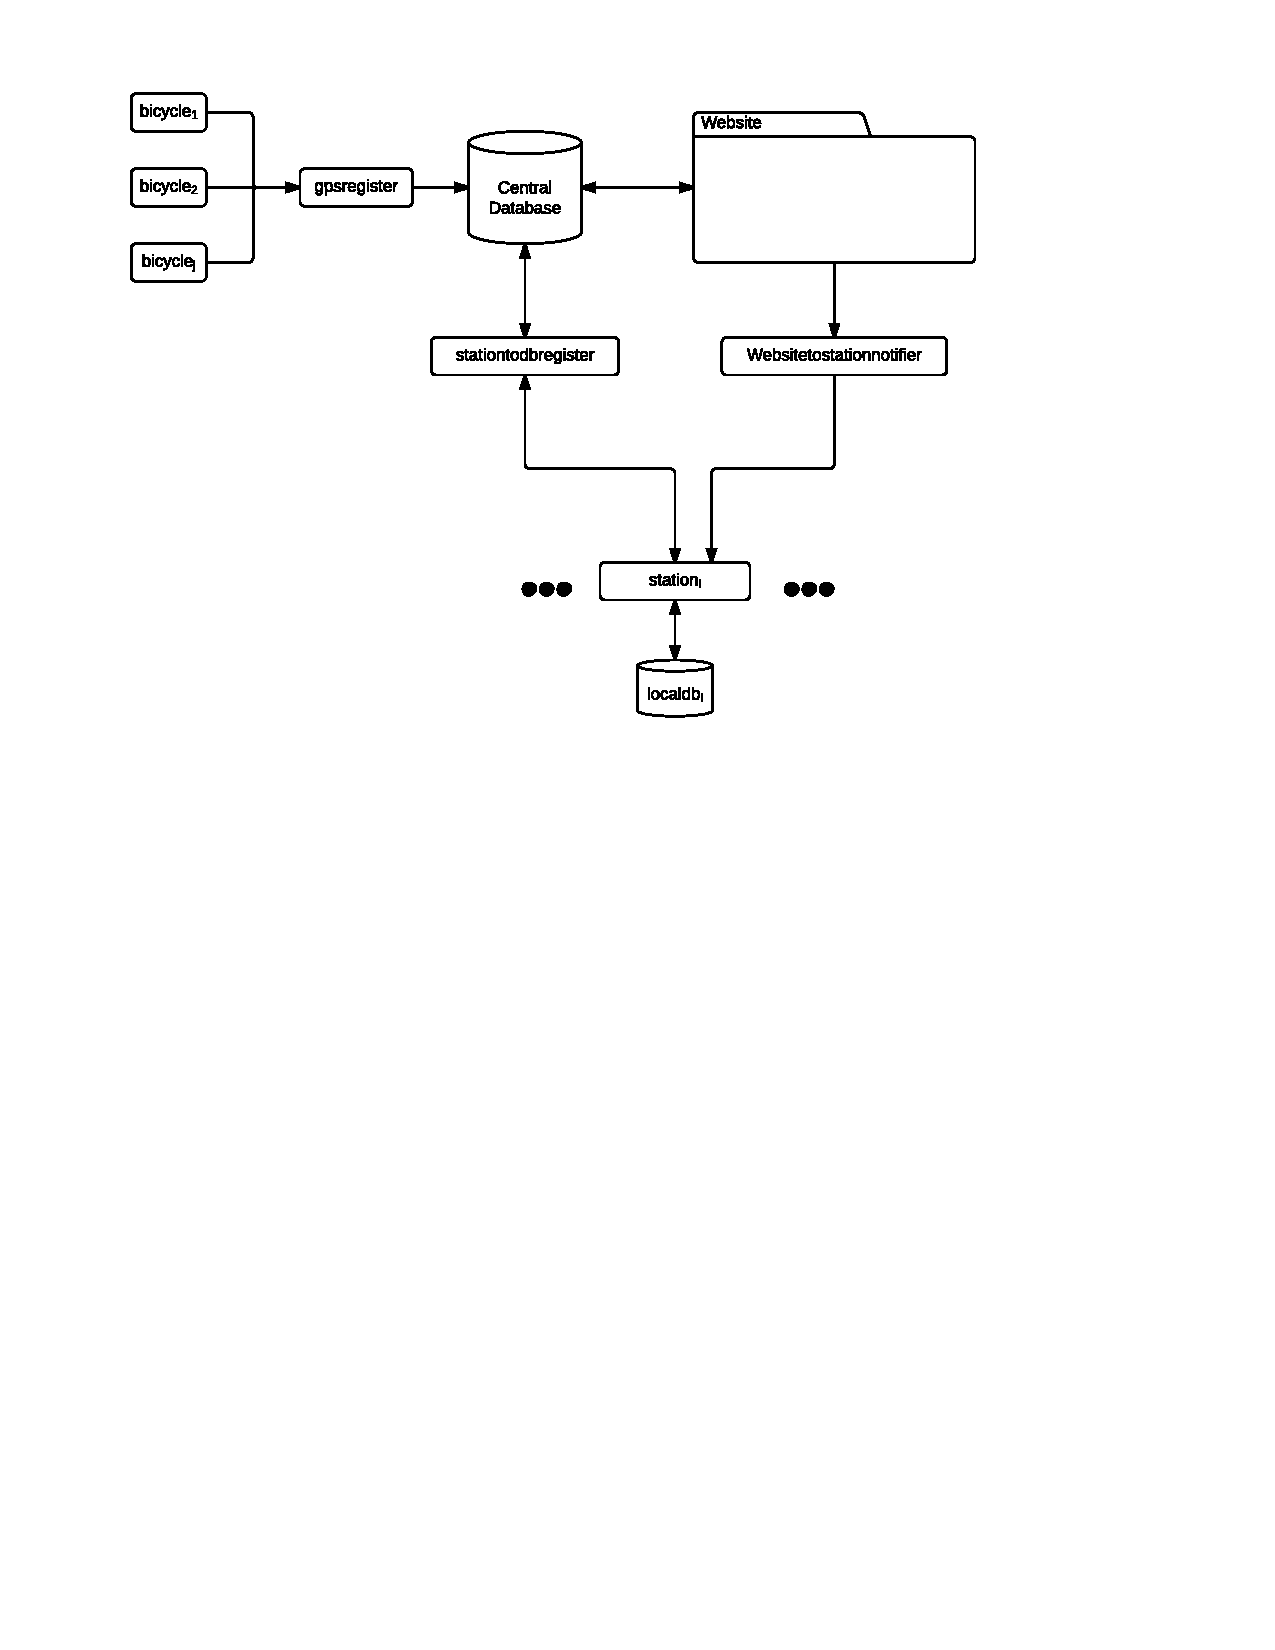
\includegraphics[trim=2cm 1.5cm 1cm 1.5cm, clip, scale=0.7]{design/architecture}
	\caption{Overall architecture}\label{fig:overallarch}
\end{figure}

As can be seen from the figure, the architecture consists of a central database as well as a website and three interfaces, named 'gpsregister´, 'stationtodbregister´, and 'websitetostationnotifier´ , where 'gpsregister´ and 'stationtodbregister´ contact the central database.
Additionally, multiple stations and their associated local database and docks exists.
The reason each station needs to have its own local database, and not merely use the central one is to minimize the necessary network communication, as well as allowing the stations to remain operational in case of network failure.
As of such, the local databases contains a subset of the central database, corresponding to the data involving the given station.
Each dock is associated with a given station, and is used by the users to take or deliver bicycles.

Additionally, the three interfaces each serves a different purpose, as described here.
The gpsregister interface, is provided for the bicycles to register their current position in the central database, as well as logging its path in another table.
This data provided can be used for route mapping and positioning of bicycles.

The stationtodbregister interface serves the purpose of updating the central database of changes performed at the local stations. Furthermore, it enables the local stations to read their subset of the central database, which is used for booting of stations from scratch, when their local database is empty.

The websitetostationnotifier is a little different, in that it is an interface provided to the website, such that when the website changes data, e.g. create a booking, the involved station is notified by the interface.

The architecture for the website is the MVC pattern, see \secref{sec:mvc}. \fxwarning{Hvilke alternativer er der?}
A detailed overview of the architecture of the controller and model part of the website are provided in \appref{app-arch:controller} and \appref{app-arch:model}

Another part of the architecture is the user interaction.
For the website, we distinguish between admin and regular users.
The admin user has access to an admin webpage, where he can modify stations, bicycles, docks, and users.
In addition to this, the admin user is also provided with some statistics pages about the usage of the system.
The admin user also has access to the features a regular user has access to.

A regular user can interact with the system in several ways.
The website allows for station status, in order to see how many bicycles and docks are available at any given station, but also the position of each station.
In addition to this, the website also provides the option to book bicycles in advance for a given station, where the station locks a bicycle some time in advance.
If you book a bicycle, you are provided with a password needed to unlock a bicycle at the station.

For the station interaction, two interactions are involved.
If you have booked a bicycle at the station in advance, you use the password provided from the website to unlock a bicycle for usage, by entering this password in the station automata.
The automata then tells you at which dock a bicycle is unlocked, and you can retrieve your bicycle.
However, if you have not booked a bicycle in advance, you do not use the station automate, but instead check each dock for available bicycles.
In that regard, we imagine a distinction between reserved unlocked bicycles and free bicycles, such that you do not on accident steal someone else's booked bicycle.

For the deliverance of bicycles, the interaction is the same whether the bicycle is booked or not.
The process is easy, as you locate a free dock and then place the bicycle at that dock.
The system will then automatically register that the bicycle has been returned to a dock at the station.

%stationer skal have egen database
%forklaring af figur
%husk teori og fancy ord, SOAP webservice er et eksempel

%uddybbelse af de enkelte komponenter.